% 2-15-rb-tree.tex

%%%%%%%%%%%%%%%%%%%%
\documentclass[a4paper, justified]{tufte-handout}

% hw-preamble.tex

% geometry for A4 paper
% See https://tex.stackexchange.com/a/119912/23098
\geometry{
  left=20.0mm,
  top=20.0mm,
  bottom=20.0mm,
  textwidth=130mm, % main text block
  marginparsep=5.0mm, % gutter between main text block and margin notes
  marginparwidth=50.0mm % width of margin notes
}

% for colors
\usepackage{xcolor} % usage: \color{red}{text}
% predefined colors
\newcommand{\red}[1]{\textcolor{red}{#1}} % usage: \red{text}
\newcommand{\blue}[1]{\textcolor{blue}{#1}}
\newcommand{\teal}[1]{\textcolor{teal}{#1}}

\usepackage{todonotes}

% heading
\usepackage{sectsty}
\setcounter{secnumdepth}{2}
\allsectionsfont{\centering\huge\rmfamily}

% for Chinese
\usepackage{xeCJK}
\usepackage{zhnumber}
\setCJKmainfont[BoldFont=FandolSong-Bold.otf]{FandolSong-Regular.otf}

% for fonts
\usepackage{fontspec}
\newcommand{\song}{\CJKfamily{song}} 
\newcommand{\kai}{\CJKfamily{kai}} 

% To fix the ``MakeTextLowerCase'' bug:
% See https://github.com/Tufte-LaTeX/tufte-latex/issues/64#issuecomment-78572017
% Set up the spacing using fontspec features
\renewcommand\allcapsspacing[1]{{\addfontfeature{LetterSpace=15}#1}}
\renewcommand\smallcapsspacing[1]{{\addfontfeature{LetterSpace=10}#1}}

% for url
\usepackage{hyperref}
\hypersetup{colorlinks = true, 
  linkcolor = teal,
  urlcolor  = teal,
  citecolor = blue,
  anchorcolor = blue}

\newcommand{\me}[4]{
    \author{
      {\bfseries 姓名:}\underline{#1}\hspace{2em}
      {\bfseries 学号:}\underline{#2}\hspace{2em}\\[10pt]
      {\bfseries 评分:}\underline{#3\hspace{3em}}\hspace{2em}
      {\bfseries 评阅:}\underline{#4\hspace{3em}}
  }
}

% Please ALWAYS Keep This.
\newcommand{\noplagiarism}{
  \begin{center}
    \fbox{\begin{tabular}{@{}c@{}}
      请独立完成作业,不得抄袭。\\
      若得到他人帮助, 请致谢。\\
      若参考了其它资料,请给出引用。\\
      鼓励讨论,但需独立书写解题过程。
    \end{tabular}}
  \end{center}
}

\newcommand{\goal}[1]{
  \begin{center}{\fcolorbox{blue}{yellow!60}{\parbox{0.50\textwidth}{\large 
    \begin{itemize}
      \item 体会``思维的乐趣''
      \item 初步了解递归与数学归纳法 
      \item 初步接触算法概念与问题下界概念
    \end{itemize}}}}
  \end{center}
}

% Each hw consists of four parts:
\newcommand{\beginrequired}{\hspace{5em}\section{作业 (必做部分)}}
\newcommand{\beginoptional}{\section{作业 (选做部分)}}
\newcommand{\beginot}{\section{Open Topics}}
\newcommand{\begincorrection}{\section{订正}}
\newcommand{\beginfb}{\section{反馈}}

% for math
\usepackage{amsmath, mathtools, amsfonts, amssymb}
\newcommand{\set}[1]{\{#1\}}

% define theorem-like environments
\usepackage[amsmath, thmmarks]{ntheorem}

\theoremstyle{break}
\theorempreskip{2.0\topsep}
\theorembodyfont{\song}
\theoremseparator{}
\newtheorem{problem}{题目}[subsection]
\renewcommand{\theproblem}{\arabic{problem}}
\newtheorem{ot}{Open Topics}

\theorempreskip{3.0\topsep}
\theoremheaderfont{\kai\bfseries}
\theoremseparator{:}
\theorempostwork{\bigskip\hrule}
\newtheorem*{solution}{解答}
\theorempostwork{\bigskip\hrule}
\newtheorem*{revision}{订正}

\theoremstyle{plain}
\newtheorem*{cause}{错因分析}
\newtheorem*{remark}{注}

\theoremstyle{break}
\theorempostwork{\bigskip\hrule}
\theoremsymbol{\ensuremath{\Box}}
\newtheorem*{proof}{证明}

% \newcommand{\ot}{\blue{\bf [OT]}}

% for figs
\renewcommand\figurename{图}
\renewcommand\tablename{表}

% for fig without caption: #1: width/size; #2: fig file
\newcommand{\fig}[2]{
  \begin{figure}[htbp]
    \centering
    \includegraphics[#1]{#2}
  \end{figure}
}
% for fig with caption: #1: width/size; #2: fig file; #3: caption
\newcommand{\figcap}[3]{
  \begin{figure}[htbp]
    \centering
    \includegraphics[#1]{#2}
    \caption{#3}
  \end{figure}
}
% for fig with both caption and label: #1: width/size; #2: fig file; #3: caption; #4: label
\newcommand{\figcaplbl}[4]{
  \begin{figure}[htbp]
    \centering
    \includegraphics[#1]{#2}
    \caption{#3}
    \label{#4}
  \end{figure}
}
% for margin fig without caption: #1: width/size; #2: fig file
\newcommand{\mfig}[2]{
  \begin{marginfigure}
    \centering
    \includegraphics[#1]{#2}
  \end{marginfigure}
}
% for margin fig with caption: #1: width/size; #2: fig file; #3: caption
\newcommand{\mfigcap}[3]{
  \begin{marginfigure}
    \centering
    \includegraphics[#1]{#2}
    \caption{#3}
  \end{marginfigure}
}

\usepackage{fancyvrb}

% for algorithms
\usepackage[]{algorithm}
\usepackage[]{algpseudocode} % noend
% See [Adjust the indentation whithin the algorithmicx-package when a line is broken](https://tex.stackexchange.com/a/68540/23098)
\newcommand{\algparbox}[1]{\parbox[t]{\dimexpr\linewidth-\algorithmicindent}{#1\strut}}
\newcommand{\hStatex}[0]{\vspace{5pt}}
\makeatletter
\newlength{\trianglerightwidth}
\settowidth{\trianglerightwidth}{$\triangleright$~}
\algnewcommand{\LineComment}[1]{\Statex \hskip\ALG@thistlm \(\triangleright\) #1}
\algnewcommand{\LineCommentCont}[1]{\Statex \hskip\ALG@thistlm%
  \parbox[t]{\dimexpr\linewidth-\ALG@thistlm}{\hangindent=\trianglerightwidth \hangafter=1 \strut$\triangleright$ #1\strut}}
\makeatother

% for footnote/marginnote
% see https://tex.stackexchange.com/a/133265/23098
\usepackage{tikz}
\newcommand{\circled}[1]{%
  \tikz[baseline=(char.base)]
  \node [draw, circle, inner sep = 0.5pt, font = \tiny, minimum size = 8pt] (char) {#1};
}
\renewcommand\thefootnote{\protect\circled{\arabic{footnote}}} % feel free to modify this file
%%%%%%%%%%%%%%%%%%%%
\title{第4-3讲: 群同态基本定理与正规子群}
\me{ 林凡琪}{211240042 }{}{}
\date{\zhtoday} % or like 2019年9月13日
%%%%%%%%%%%%%%%%%%%%
\begin{document}
\maketitle
%%%%%%%%%%%%%%%%%%%%
\noplagiarism % always keep this line
%%%%%%%%%%%%%%%%%%%%
\begin{abstract}
	% \begin{center}{\fcolorbox{blue}{yellow!60}{\parbox{0.65\textwidth}{\large 
	%   \begin{itemize}
	%     \item 
	%   \end{itemize}}}}
	% \end{center}
\end{abstract}
%%%%%%%%%%%%%%%%%%%%
\beginrequired

%%%%%%%%%%%%%%%
\begin{problem}[TJ 9-11]
\end{problem}

\begin{solution}
	$Z/8Z, (Z/4Z) \times (Z/2Z), (Z/2Z) \times (Z/2Z) \times (Z/2Z)$, $D4$ (or $D8$) and the quaternion group $Q8$.
\end{solution}
%%%%%%%%%%%%%%%

%%%%%%%%%%%%%%%
\begin{problem}[TJ 9-16]
\end{problem}

\begin{solution}
	The order of an element in a direct product of groups is the least common multiple of the orders of its components.\\
	(a)the order of (3, 4) in $Z_4 \times Z_6$ is lcm(4, 6) = 12.\\
	(b) The order of (6, 15, 4) in $Z_{30} \times Z_{45} \times Z_{24}$ is lcm(5, 3, 6) = 30.\\
	(c)The order of (5, 10, 15) in $Z_{25} \times Z_{25} \times Z_{25}$ is lcm(5, 5, 5) = 5. \\
	(d) The order of (8, 8, 8) in $Z_{10} \times Z_{24} \times Z_{80}$ is lcm(5, 3, 10) = 30.
\end{solution}
%%%%%%%%%%%%%%%

%%%%%%%%%%%%%%%
\begin{problem}[TJ 9-23]
\end{problem}

\begin{solution}
	The assertion is false.\\
	Disproof:\\
	A counterexample is given by $G = Z_2 × Z_4, H = Z_4 × Z_2$, and $K = Z_2$. Then $G × K \cong  H × K \cong Z_2 × Z_4 × Z_2$, but $G \cong H$. This is because the direct product of groups is commutative and associative up to isomorphism, but the order of factors matters for the isomorphism type of the group.
\end{solution}
%%%%%%%%%%%%%%%

%%%%%%%%%%%%%%%
\begin{problem}[TJ 10-1(a,c)]
\end{problem}

\begin{solution}
	A subgroup H of a group G is normal if and only if $gH = Hg$ for all $g \in G$. This means that every left coset of H is equal to a right coset of H. Equivalently, H is normal if and only if $ghg^{-1} \in H$ for all $g \in G$ and $h \in H$. This means that aevery element of H is conjugate to itself by any element of G.

	(a) The subgroup $A_4$ of $S_4$ is normal because it is the kernel of the sign homomorphism from $S_4$ to $Z_2$. Alternatively, we can check that every element of $A_4$ is conjugate to itself by any element of $S_4$. For example, $(1 2 3)(1 4)(1 2 3)^{-1} = (1 3 4)$ is in $A_4$. The factor group $S_4/A_4$ has order 2 and consists of the cosets $A_4$ and $(1 2)A_4$. The Cayley table for $S_4/A_4$ is:

	\[ \begin{array}{c|cc} & A_4 & (1 2)A_4 \\ \hline A_4 & A_4 & (1 2)A_4 \\ (1 2)A_4 & (1 2)A_4 & A_4 \end{array} \]

	(c) The subgroup $D_4$ of $S_4$ is not normal because it is not invariant under conjugation by some elements of $S_4$. For example, $(1 3)(1 2)(1 3)^{-1} = (2 3)$ is not in $D_4$. Therefore, we cannot form a factor group $G/H$ in this case.
\end{solution}
%%%%%%%%%%%%%%%

%%%%%%%%%%%%%%%
\begin{problem}[TJ 10-11]
\end{problem}

\begin{solution}
	Let g be any element of G and let h be any element of H. Then $ghg^(-1)$ is also an element of G with order k, since $(ghg(-1))k = ghkg(-1) = g1g^(-1) = 1$. Therefore, $ghg^(-1)$ must belong to H, since $H$ is the only subgroup of $G$ with order $k$. This shows that $H$ is normal in $G$.
\end{solution}
%%%%%%%%%%%%%%%


%%%%%%%%%%%%%%%
\begin{problem}[TJ 10-12]
\end{problem}

\begin{solution}

	The centralizer of an element $g$ in a group $G$ is the set of elements of $G$ that commute with $g$, or in other words, that satisfy $xg = gx$ for any $x$ in $C(g)$. To show that $C(g)$ is a subgroup of $G$, we need to check three conditions:

	- $C(g)$ is non-empty. This is true because $g$ belongs to $C(g)$, since $gg = gg$.

	- $C(g)$ is closed under the group operation. This means that if $x$ and $y$ belong to $C(g)$, then $xy$ also belongs to $C(g)$. To see this, note that $(xy)g = x(yg) = x(gy) = (xg)y = (gx)y = g(xy)$, using the fact that $x$ and $y$ commute with $g$.

	- $C(g)$ is closed under taking inverses. This means that if $x$ belongs to $C(g)$, then $x^{-1}$ also belongs to $C(g)$. To see this, note that $x^{-1} g = (xg)^{-1} = (gx)^{-1} = g^{-1} x^{-1} = x^{-1} g^{-1}$, using the fact that $x$ commutes with $g$ and the inverse property.

	Therefore, $C(g)$ is a subgroup of $G$. If $g$ generates a normal subgroup of $G$, then we need to show that $C(g)$ is normal in $G$. This means that for any $x$ in $G$ and $y$ in $C(g)$, we have $xyx^{-1}$ in $C(g)$. To see this, note that $(xyx^{-1}) g = xygx^{-1} = xyx^{-1} xg = yg$, using the fact that y commutes with g and the inverse property. Similarly, $(gxyx^{-1}) = gyx^{-1} = yx^{-1} gx^{-1} = xyx^{-1} g$. Therefore, $(xyx^{-1})$ commutes with g and belongs to C(g).

\end{solution}
%%%%%%%%%%%%%%%


%%%%%%%%%%%%%%%
\begin{problem}[TJ 11-5]
\end{problem}

\begin{solution}
	A homomorphism from $Z_{24}$ to $Z_{18}$ is a function that preserves the group operation, that is, $f(x+y) = f(x) + f(y)$ for any $x,y \in Z_{24}$. Such a function is completely determined by the value of $f(1)$, since $f(n) = n f(1)$ for any $n \in Z_{24}$. Moreover, the value of $f(1)$ must satisfy two conditions:

	-It must be an element of $Z_{18}$, that is, an integer between $0$ and $17$.

	-It must divide $24$, that is, it must be a multiple of $3$.

	The second condition follows from the fact that the order of $f(1)$ in $Z_{18}$ must divide the order of $1$ in $Z_{24}$, which is $24$. Therefore, there are only six possible values for $f(1)$: $0$, $3$, $6$, $9$, $12$, and $15$. For each of these values, we can define a homomorphism by

	$$f_k(n) = 3kn \mod 18$$

	where $k$ is the value of $f(1)$. For example, if $f(1) = 9$, then

	$$f_9(n) = 27n \mod 18 = 9n \mod 18$$

	These are all the homomorphisms from $Z_{24}$ to $Z_{18}$.


\end{solution}
%%%%%%%%%%%%%%%

%%%%%%%%%%%%%%%
\begin{problem}[TJ 11-2(b,d,e)]
Which of the following maps are homomorphisms? If the map is a homomorphism,
what is the kernel?
(b)$\phi: \mathbb{R} \rightarrow G L_2(\mathbb{R})$ defined by
$$
	\phi(a)=\left(\begin{array}{ll}
			1 & 0 \\
			a & 1
		\end{array}\right)
$$

(d)$\phi: G L_2(\mathbb{R}) \rightarrow \mathbb{R}^*$ defined by
$$
	\phi\left(\left(\begin{array}{ll}
				a & b \\
				c & d
			\end{array}\right)\right)=a d-b c
$$
(e)
$\phi: \mathbb{M}_2(\mathbb{R}) \rightarrow \mathbb{R}$ defined by
$$
	\phi\left(\left(\begin{array}{ll}
				a & b \\
				c & d
			\end{array}\right)\right)=b,
$$
where $\mathbb{M}_2(\mathbb{R})$ is the additive group of $2 \times 2$ matrices with entries in $\mathbb{R}$.
\end{problem}

\begin{solution}
	一个同态映射是一个保持群运算的映射,即$\phi(g_1g_2) = \phi(g_1)\phi(g_2)$,其中$g_1,g_2$是群的元素。一个同态映射的核是所有映到群的单位元的元素组成的集合,即$\ker(\phi) = {g \in G | \phi(g) = e}$,其中$e$是群的单位元。核是一个群的子群。


	(b) $\phi: \mathbb{R} \rightarrow G L_2(\mathbb{R})$是一个同态映射.\\
	因为
	$$
		\begin{aligned}
			\phi(a+b)                                                    & =
			\left(\begin{array}{ll} 1 &
             0        \\ a+b &
             1
			      \end{array}\right)                                                     \\  & =\left(\begin{array}{ll} 1 & 0 \\ a & 1 \end{array}\right)
			\left(\begin{array}{ll} 1 & 0 \\ b & 1 \end{array}\right) \  & =\phi(a) \phi(b)\end{aligned} $$ 它的核是$\ker(\phi) = {0}$,因为只有当$a=0$时,$\phi(a)$才是$GL_2(\mathbb{R})$的单位元。

	(d) $\phi: G L_2(\mathbb{R}) \rightarrow \mathbb{R}^*$是一个同态映射,因为
	$$
		\begin{aligned}                                                                                                           &
                                                                                                                        \phi\left(\left(\begin{array}{ll} a_{1} & b_{1} \\
             c_{1}      & d_{1}
				                                                                                                                                        \end{array}\right)
                                                                                                                        \left(\begin{array}{ll} a_{2} & b_{2} \\
             c_{2}      & d_{2}\end{array}\right)\right)                                                   \\
                                                                                                                        = & \phi\left(\left(\begin{array}{ll} a_{1} a_{2}+b_{1} c_{2} & a_{1} b_{2}+b_{1} d_{2} \\
             c_{1} a_{2}+d_{1} c_{2}      & c_{1} b_{2}+d_{1} d_{2}\end{array}\right)\right) \\
                                                                                                                        = & (a_{1} a_{2}+b_{1} c_{2})(c_{1} b_{2}+d_{1} d_{2})-(a_{1} b_{2}+b_{1} d_{2})(c_{1} a_{2}+d_{1} c_{2})                                                                                                                   \\
                                                                                                                        = & (a_1d_1-b_1c_1)(a_2d_2-b_2c_2)                                                                                                                                                                                          \\
                                                                                                                        = & \phi\left(\left(\begin{array}{ll} a_{1} & b_{1} \\
             c_{1}      & d_{1}\end{array}\right)\right)
                                                                                                                        \phi\left(\left(\begin{array}{ll} a_{2} & b_{2} \\
             c_{2}      & d_{2}\end{array}\right)\right)
		\end{aligned} $$
	它的核是$\ker(\phi) = SL_2(\mathbb{R})$,即所有行列式为$1$的矩阵组成的集合。

	(e) $\phi: \mathbb{M}_2(\mathbb{R}) \rightarrow \mathbb{R}$不是一个同态映射。要看到这一点,让 $A, B \in \mathbb{M}_2(\mathbb{R})$ 并计算:

	$$ \phi(A + B) = \phi\left(\left(\begin{array}{ll} a_1 & b_1 \\
             c_1      & d_1\end{array}\right) + \left(\begin{array}{ll} a_2 & b_2 \\
             c_2      & d_2\end{array}\right)\right) = \phi\left(\left(\begin{array}{ll} a_1 + a_2 & b_1 + b_2 \\
             c_1 + c_2      & d_1 + d_2\end{array}\right)\right) $$

	$$ = b_1 + b_2 $$

	但是

	$$ \phi(A) + \phi(B) = b_1 + b_2 $$

	所以,$\phi(A + B) = \phi(A) + \phi(B)$ 只有当 $b_1 = b_2 = 0$ 时才成立,这对于 $\mathbb{M}_2(\mathbb{R})$ 中的所有矩阵都不成立。因此,$\phi$ 不是同态。

	由于 $\phi$ 不是同态,$\phi$ 的核不是良定义的。然而,如果我们仍然想要找到被 $\phi$ 映射到零的矩阵的集合,我们需要解 $\phi(A) = 0$,其中 $A$ 是一个 $2 \times 2$ 矩阵。这给我们 $b = 0$,所以集合是形式为 $\left(\begin{array}{ll} a & 0 \\ c & d \end{array}\right)$ 的矩阵的集合,其中 $a, c, d \in \mathbb{R}$。


\end{solution}
%%%%%%%%%%%%%%%


%%%%%%%%%%%%%%%%%%%%
\beginoptional

%%%%%%%%%%%%%%%

%%%%%%%%%%%%%%%
\begin{problem}[SageMath学习]
学习 TJ 第9、10/11章 关于 SageMath 的内容
\end{problem}

\begin{solution}
\end{solution}
%%%%%%%%%%%%%%%

%%%%%%%%%%%%%%%
\begin{problem}[TJ 11-17]
\end{problem}

\begin{solution}
\end{solution}
%%%%%%%%%%%%%%%


%%%%%%%%%%%%%%%
\begin{problem}[6、8阶群]
请给出同构意义下的所有6阶、8阶群。
\end{problem}

\begin{solution}
	同构意义下的所有6阶群,两种:循环群和三元对称群。
	同构意义下的所有8阶群,五种:循环群、四元数群、二阶循环群的直积、二阶循环群的半直积和二阶对称群。
\end{solution}
%%%%%%%%%%%%%%%

%%%%%%%%%%%%%%%%%%%%
\beginot
%%%%%%%%%%%%%%%
\begin{ot}[群同态第二定理]
	请证明群同态第二定理。
\end{ot}

% \begin{solution}
% \end{solution}
%%%%%%%%%%%%%%%

%%%%%%%%%%%%%%%

\begin{ot}[同态猜想]


	\begin{minipage}{\linewidth}

		\centering
		\vspace{5cm}
		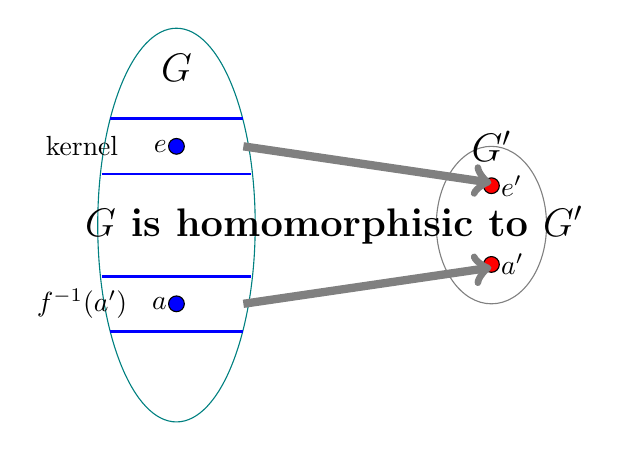
\begin{tikzpicture}

			\draw  (-2,1) [fill=blue]circle (0.1) node [left] {$e$};
			\draw  (-2,-1) [fill=blue]circle (0.1) node [left] {$a$};

			\draw (-2,0)[color=teal]circle (1 and 2.5);

			\draw   [ color=blue, line width=1pt] (-2.95,0.65)--(-1.05,0.65);
			\draw   [ color=blue, line width=1pt] (-2.85,1.35)--(-1.15,1.35);

			\draw   [ color=blue, line width=1pt] (-2.95,-0.65)--(-1.05,-0.65);
			\draw   [ color=blue, line width=1pt] (-2.85,-1.35)--(-1.15,-1.35);

			\draw  (2,0.5) [fill=red]circle (0.1) node (e1)[right]{$e'$};
			\draw  (2,-0.5) [fill=red]circle (0.1) node (a1)[right]{$a'$};

			\draw (2,0) [color= gray] circle (0.7 and 1);

			\draw [->,color=gray,line width=3pt,] (-1.15,1) to (e1);
			\draw [->,color=gray,line width=3pt,] (-1.15,-1) to (a1);

			\node at(-3.2,1){kernel};
			\node at (-3.2,-1){$f^{-1}(a')$};

			\node at (-2,2) {\Large \textbf{$G$}};

			\node at (2,1) {\Large \textbf{$G'$}};


			\node at (0,0) {\Large \textbf{$G \text{ is homomorphisic to } G'$}};
		\end{tikzpicture}
	\end{minipage}

	请证明或证否下列猜想
	\begin{itemize}
		\item Kernel和任意的$G'$中非单位元元素的逆像不相交
		\item Kernel和任意的$G'$中非单位元元素的逆像同势
		\item 任意的$G'$中元素的逆像不相交且同势
		\item 任意的$G'$中元素的逆像必定是kernel的某个陪集

	\end{itemize}
\end{ot}


% \begin{solution}
% \end{solution}
%%%%%%%%%%%%%%%


% \vspace{0.50cm}
%%%%%%%%%%%%%%%
% \begin{ot}[]
% 
%   \noindent 参考资料:
%   \begin{itemize}
%     \item 
%   \end{itemize}
% \end{ot}

% \begin{solution}
% \end{solution}
%%%%%%%%%%%%%%%

%%%%%%%%%%%%%%%%%%%%
% 如果没有需要订正的题目,可以把这部分删掉

% \begincorrection
%%%%%%%%%%%%%%%%%%%%

%%%%%%%%%%%%%%%%%%%%
% 如果没有反馈,可以把这部分删掉
\beginfb

% 你可以写
% ~\footnote{优先推荐 \href{problemoverflow.top}{ProblemOverflow}}:
% \begin{itemize}
%   \item 对课程及教师的建议与意见
%   \item 教材中不理解的内容
%   \item 希望深入了解的内容
%   \item $\cdots$
% \end{itemize}
%%%%%%%%%%%%%%%%%%%%
% \bibliography{2-5-solving-recurrence}
% \bibliographystyle{plainnat}
%%%%%%%%%%%%%%%%%%%%
\end{document}